\chapter{Fundamentación y teoría}
\label{sec:Fundamentacion}

\section{Concurrencia}

La concurrencia en sistemas se puede manifestar en la capacidad que tiene el sistema de gestionar múltiples tareas o flujos de datos a la vez, sin que uno tenga que terminar necesariamente para que otra tarea comience. En esta sección se hablará de cómo Steam tiene procesos concurrentes y en qué funcionalidades se puede observar esto.

\textbf{Desacoplamiento: } El modelo de Steam se basa principalmente en conexiones uno a uno de cliente-servidor, pero incluso en estas conexiones existen procesos concurrentes. Esto se puede ver reflejado en, por ejemplo, si un usuario está ejecutando una tarea de enviar un mensaje, el servidor puede estar procesando otro mensaje que envió otro usuario, haciendo este proceso un proceso concurrente y no iterativo, ya que el segundo usuario pudo mandar el mensaje sin que tuviera que esperar a que se procese el mensaje del primer usuario. Gracias al buffer que el sistema posee, se permite que el flujo de salida del usuario y el flujo de procesamiento del servidor ocurran de forma concurrente en vez de manera iterativa o secuencial.

\textbf{Concurrencia en la capa de transporte TCP/IP: } El protocolo TCP/IP maneja igualmente la concurrencia, aunque de menor nivel. Mientras Steam está mandando datos, el sistema operativo, simultáneamente realiza más procesos como pueden ser el encapsulamiento de datos en segmentos, la gestión de envíos de ACKs técnicos (ACK son mensajes de confirmación) y el control de flujo de la ventana, para que no sature al receptor.

\textbf{Servidor, entidad concurrente: } El servidor, como sistema real usa \textit{threads} para manejar la concurrencia de usuarios, esto hace que múltiples usuarios estén conectados simultáneamente y puedan usar funcionalidades, por cada usuario que se conecte se genera un \textit{thread} independiente, para que el procesamiento de datos de un usuario que vaya lento no bloquee la entrada a otros usuarios que también quieran usar esas funcionalidades.

La mayoría de las funcionalidades concurrentes de Steam son gracias a la integración de un buffer que permite que se procesen datos a una velocidad equilibrada. Un buffer es un espacio de memoria física o virtual que se utiliza en servidores para almacenar temporalmente datos mientras se transfieren. Esto generalmente se ve representado como una cola, que evita interrupciones en la transmisión de la información entre dispositivos o servidores.

\section{Posibles fallos en nodos independientes}

En todos los sistemas existen fallos que pueden ocasionar que se pueda caer todo el sistema por algun nodo importante, por eso se trata de construir sistemas que tengan nodos independientes y que no conlleven que se caiga todo si es que llega a fallar. Los fallos de nodos independientes son críticos igualmente en sistemas distribuidos, porque el sistema no puede distinguir entre un proceso caído y uno lento.

\textbf{Fallos en nodos de usuario: } Pueden existir fallos en los nodos que serían los usuarios de Steam, estos fallos pueden ser de red o de hardware (aunque también de software). Algunos ejemplos de fallos que se pueden ocasionar son que se le vaya la luz al usuario, que el sistema operativo del usuario le de un pantallazo azul o algún fallo interno de hardware, como que se le queme el procesador u otro componente del computador.

\begin{figure} [h] % [h]
	\centering
	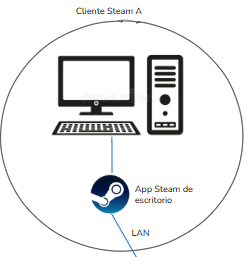
\includegraphics[width=0.4\textwidth]{Figuras/nodousuario}
	\caption{Representación usuario}
\end{figure}


\textbf{Fallos en nodos de infraestuctura de redes: } Algún posible fallo que se podría identificar en la infraestructura de red es que se sobrecaliente el Router, o se vaya la luz, imposibilitando el enrutamiento del usuario. Esto tendría un impacto inmediato porque el usuario queda incomunicado con el sistema y aislado del mundo exterior.

\begin{figure} [h] % [h]
	\centering 
	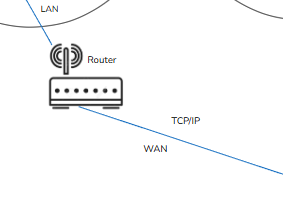
\includegraphics[width=0.4\textwidth]{Figuras/nodorouter}
	\caption{Representación nodo infraestructura de red}
\end{figure}


\textbf{Fallos en nodos de servicio: 	} Pueden fallar los dispositivos que componen las bases de datos de los servidores, esto generaría impactos en las funcionalidades, en temas de tiempo más que nada, ya que como se observa en la Figura 3 los dispositivos que componen la base de datos están en topología de estrella, por lo que si uno falla, los demás pueden funcionar normalmente, y así no afectaría a las funcionalidades que ofrecen. Además, el sistema cuenta con servidores de respaldo, por lo que refuerza lo que se dijo antes de que no afectaría.

\begin{figure}[H]
	\centering
	\includegraphics[width=0.2\textwidth]{Figuras/bdd}
	\caption{Representación servidor}
\end{figure}

\section{Justificación de transparencia}

Para justificar la transparencia en el sistema propuesto, es necesario analizar cómo el diseño oculta la complejidad de la red y la distribución geográfica, permitiendo que el usuario e incluso los admins interactúen con el sistema como si fuera una única entidad local.

En esta parte se detallará cómo se logran estas transparencias integrando los modelos y el contexto de los servicios de Steam.

\textbf{Transparencia de acceso: } Este tipo de transparencia garantiza que la forma en la cuál se puede acceder a un recurso sea la misma, esto si es remoto o local. La comunicación se centraliza en el uso de sockets como \textit{endpoints}. La abstracción oculta si el mensaje viaja por la memoria del sistema o si va por la red. Cuando un usuario envía un mensaje al chat, la interfaz de Steam no cambia si el servidor de mensajería está en su ciudad o si está en otro lugar. La transparencia de acceso de Steam se logra porque la capa de aplicación delega en el \textit{middleware} la tarea de hacer el \textit{marshalling} de los datos, convirtiéndolos en un formato accesible para que el protocolo TCP/IP pueda funcionar sin que el usuario tenga que intervenir para esto.

\textbf{Transparencia de ubicación: } Esta transparencia permite acceder a los recursos (que pueden ser archivos, servidores, bases de datos) sin la necesidad de conocer su ubicación física (direccion IP o rack). En la Figura 4 se observa que los usuarios están separados de los servidores por múltiples saltos. La transparencia de ubicación se logra porque el cliente no necesita conocer la ruta física ni en qué puerto del switch está conectada la Base de Datos, por lo que usa identificadores lógicos o en su defecto nombres de servicio. El usuario al realizar una compra de un juego/producto, inicia un proceso síncrono (similar a un RPC), el usuario simplemente interactúa con la tienda, mientras que el sistema resuelve dinámicamente si la petición debe ir a un servidor con una zona horaria específica para optimizar la carga, y esto mantiene la ubicación física del servidor totalmente invisible para el usuario.

\begin{figure}[h]
	\centering
	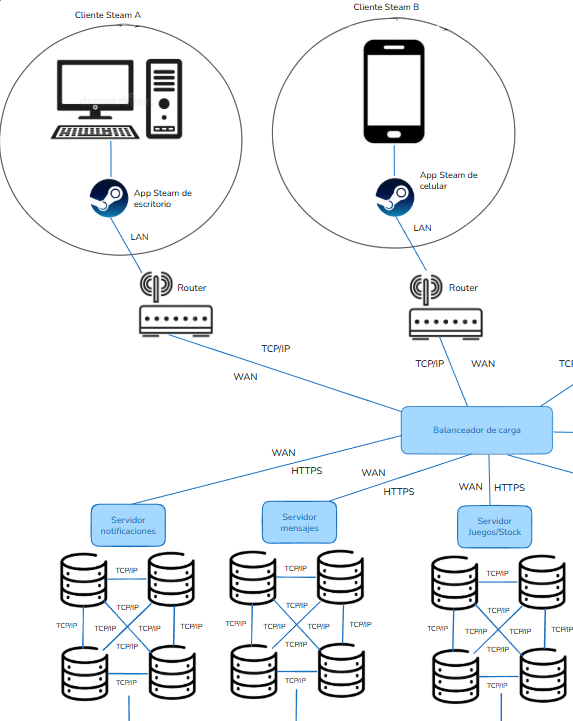
\includegraphics[width=0.5\textwidth]{Figuras/fisicoservidores}
	\caption{Usuarios y servidores}
\end{figure}

La implementación logra estas transparencias al desacoplar la lógica del negocio de la infraestructura de red. Mientras que el modelo físico define dónde están las máquinas y los firewalls , los modelos de comunicación síncronos y asíncronos definen cómo fluyen los mensajes a través de interfaces uniformes. Esto asegura que, aunque un servidor de Steam se mueva o cambie su configuración interna, el acceso y la experiencia para el usuario final permanezcan inalterados.

